\documentclass[a4paper]{article}
\usepackage[english]{babel}
\usepackage[utf8]{inputenc}
\usepackage{textcomp}
\usepackage{amsmath}
\usepackage{gensymb}
\usepackage{physics}
\usepackage{graphicx}
\usepackage[colorinlistoftodos]{todonotes}
\usepackage[margin=0.5in]{geometry}
\usetikzlibrary{quotes,angles}
\usetikzlibrary{decorations.pathreplacing}
\usetikzlibrary{calc}

\title{Notes}
\author{David Behrle}
\let\phi\varphi
\let\bf\textbf
 
\begin{document}
\maketitle
\section{Chapter 1}
    \subsection{Order of magnitude}

    The order of magnitude of a number is the power of 10 that most closely approximates it. To find the order of magnitude of a number, take the base-10 log and round to the nearest integer, the order of magnitude for the number is simply the resulting power of 10. The order of magnitude of 800 is $10^3$ because $\log_{10}800 \approx 2.903$ which rounds to 3. The order of magnitude of 250 is $10^2$ because $\log_{10}250 \approx 2.397$ which rounds to 2.
    
    On a log base-10 scale, $\sqrt{10} = 10^{\frac{1}{2}}$ is halfway between $10^0 = 1$ and $10^1 = 10$.It is quicker to write a number in scientific notation and see whether the first factor is greater than or less than $\sqrt{10} \approx 3.162$. If the first factor is less than $\sqrt{10}$, round it down to 1, and the order of magnitude is the power of 10 required to write it in scientific notation If the first factor is greater than $\sqrt{10}$, round it up to 10, and the order of magnitude is one more than the power needed to write the number in scientific notation. For example $800 = 8 \cdot 10^2$; because $8 > \sqrt{10} \approx 3.162$, the order of magnitude of 800 is $10^{2+1} = 10^3$. $250 = 2.5 \cdot 10^2$ and $2.5 < \sqrt{10}$ the order of magnitude of 250 is $10^2$.

    \subsection{Unit conversion}

    If the distance from university to home is 10 miles and it takes 20 minutes to drive this distance, calculate the average speed in meters per second (m/s, ms$^{-1}$) (distance travelled over travel time)

    \begin{equation}
        \text{Average speed} = \frac{\text{distance}}{\text{time}} = \frac{s}{t} = \frac{10 \text{ mi}}{20 \text{ min}} = 0.5 \frac{\text{mi}}{\text{min}}
    \end{equation}
    \begin{equation}
        0.5 \frac{\text{ mile}}{\text{ minute}} \cdot \frac{1609 \text{ m}}{1 \text{ mile}} \cdot \frac{1 \text{ minute}}{60 \text{ seconds}} = \frac{(1609)(0.5)}{60} \text{m/s} = 13 \text{ms$^{-1}$}
    \end{equation}

    \subsection{Dimensional analysis}

    \begin{itemize}
        \item Length = L
        \item Mass = M
        \item Time = T
        \item Current = I
        \item Thermodynamic temperature = $\theta$
        \item Amount of substance = N
        \item Luminous intensity = J
    \end{itemize}
    Physicists often use square brackets around the symbol for a physical quantity to represent the dimensions of that quantity. If $r$ is the radius of a cylinder and $h$ is its height, [$r$] = L and [$h$] = L are used to indicate the dimensions of radius and height are both length or L. Similarly for area and volume, [$A$] = L$^2$ and [$V$] = L$^3$. If the symbol $m$ is used for mass of the cylinder and $\rho$ for the density of the material, then [$m$] = M and [$\rho$] = ML$^{-3}$

    Consider the physical quantities $s$, $v$, $a$, and $t$ with the dimensions [$s$] = L, [$v$] = LT$^{-1}$, [$a$] = LT$^{-2}$, and [$t$] = T. Determine whether each of the following equations is dimensionally consistent: (a) $s = vt + 0.5at^2$; (b) $s = vt^2 + 0.5at$; (c) $v = \sin\big(\frac{at^2}{s}\big)$

    \begin{equation}
        \text{(a) } s = vt + 0.5at^2
    \end{equation}
    \begin{equation}
        [s] = \text{L}
    \end{equation}
    \begin{equation}
        [vt] = [v] \cdot [t] = \text{LT$^{-1}$} \cdot \text{T} = \text{LT$^0$} = \text{L}
    \end{equation}
    \begin{equation}
        [0.5at^2] = [a] \cdot [t]^2 = \text{LT$^{-2}$} \cdot \text{T$^2$} = \text{LT$^0$} = \text{L}
    \end{equation}
    (a) is dimensionally consistent

    \begin{equation}
        \text{(b) } s = vt^2 + 0.5at
    \end{equation}
    \begin{equation}
        [s] = \text{L}
    \end{equation}
    \begin{equation}
        [vt^2] = [v] \cdot [t]^2 = \text{LT$^{-1}$} \cdot \text{T$^2$} = \text{LT}
    \end{equation}
    \begin{equation}
        [0.5at] = [a] \cdot [t] = \text{LT$^{-2}$} \cdot \text{T} = \text{LT$^{-1}$}
    \end{equation}
    (b) is not dimensionally consistent, none of the terms has the same dimension

    \begin{equation}
        \text{(c) } v = \sin\bigg(\frac{at^2}{s}\bigg)
    \end{equation}
    (make sure the argument for the sine function is dimensionless)
    \begin{equation}
        \bigg[\frac{at^2}{s}\bigg] = \frac{[a] \cdot [t]^2}{[s]} = \frac{(\text{LT$^{-2}$}) \text{(T$^2$)}}{\text{L}} = \frac{\text{L}}{\text{L}} = 1
    \end{equation}
    \begin{equation}
        [v] = \text{LT$^{-1}$}
    \end{equation}
    \begin{equation}
        \bigg[\sin\bigg(\frac{at^2}{s}\bigg)\bigg] = 1
    \end{equation}
    (c) is not dimensionally consistent, none of the terms has the same dimension

    The derivative of a function is just the slope of the line tangent to its graph; slopes are ratios, so for physical quantities $v$ and $t$, the dimension of $v'$ with respect to $t$ is the ratio of the dimension of $v$ over that of $t$
    \begin{equation}
        \bigg[\frac{dv}{dt}\bigg] = \frac{[v]}{[t]}
    \end{equation}
    Because integrals are just sums of products, the dimension of the the integral of $v$ with respect to $t$ is the dimension of $v$ times $t$
    \begin{equation}
        \bigg[\int vdt\bigg] = [v] \cdot [t]
    \end{equation}

    \subsection{Estimates and Fermi calculations}
    Estimate the total mass of the Earth's oceans. For H$_2$O, $\rho = 10^3 \text{kg/m$^3$}$. The volume of the oceans can be estimated as the surface area times average depth, $V = AD$. The surface area of the  earth can roughly approximate the surface area of the oceans, the diameter of the earth is roughly $10^7$m. Surface area can be estimated using the surface area of a sphere $A = \pi d^2$. The average depth of the oceans can be ballparked by knowing that the deepest points are around 10 km and that it is not uncommon for the ocean to be deeper than 1 km, taking the average depth to be around $(10^3 \cdot 10^4)^{\frac{1}{2}} \approx 3\cdot 10^3$m. First, surface area is estimated
    \begin{equation}
        A = \pi d^2 = \pi (10^7\text{m})^2 \approx 3 \cdot 10^{14} \text{m}^2
    \end{equation}
    Then using the average depth estimate $D = 3 \cdot 10^3$m, volume is estimated
    \begin{equation}
        V = AD = (3 \cdot 10^{14}\text{m}^2)(3 \cdot 10^3\text{m}^2) = 9 \cdot 10^{17}\text{m}^3
    \end{equation}
    Finally, the mass of the oceans is estimated
    \begin{equation}
        M = \rho V = (10^3\text{kg/m}^3)(9 \cdot 10^{17}\text{m}^3) = 9 \cdot 10^{20}\text{kg}
    \end{equation}
    Concluding that the order of magnitude of the mass of the Earth's oceans is $10^{21}$kg

    \section{Chapter 2}
    \subsection{Scalars and Vectors}
    Scalar quantities are physical quantities that can be specified completely by giving a number and appropriate unit (time, mass distance, length, volume, temperature, and energy). Scalar quantities with the same units can be added, subtracted, or multiplied by a number normally. Two different scalar quantities can be multiplied or divided by each other to form a derived scalar quantity (g/mol, m/s$^2$, km/h, etc.) 
    
    Vector quantities cannot be completely described with just a number and physical unit, and require a directional component. Vectors have... 
    % finish later

    \subsection{Coordinate Systems and Vector Components}

    \begin{center}
    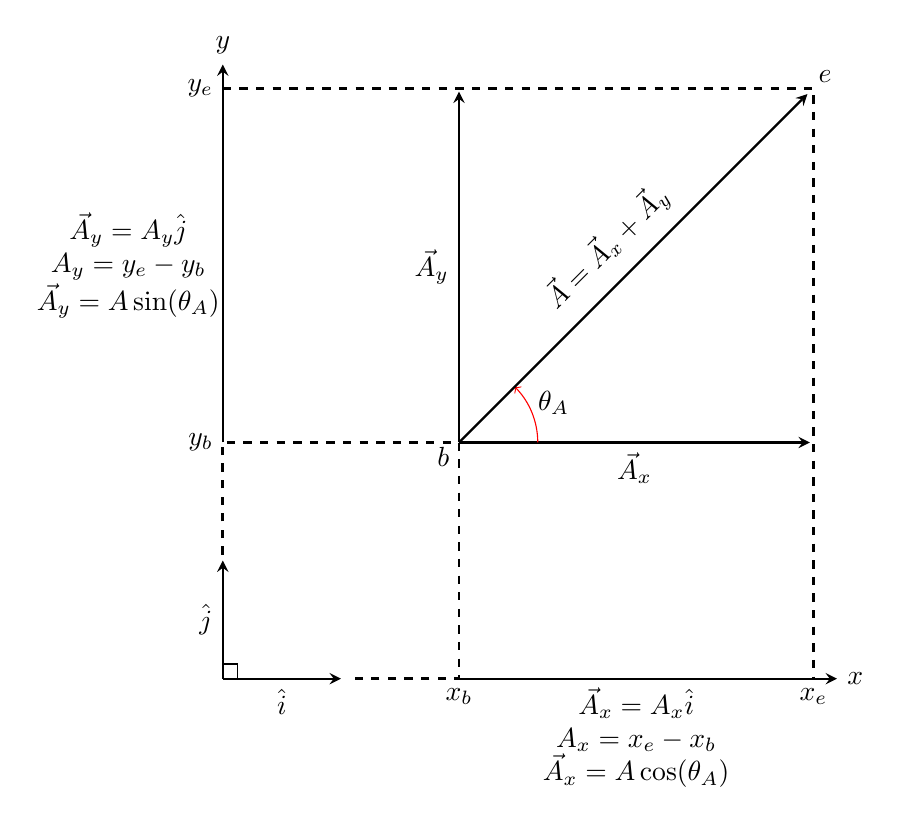
\begin{tikzpicture}[scale=1.5]
        %%%COMPONENTS%%%
        \draw[->, thick, -stealth] (0,0)--node[below]{$\hat{i}$}(1,0);
        \draw[->, thick, -stealth] (0,0)--node[left]{$\hat{j}$} (0,1);
        \draw[line width=0.5pt] (0,0.125)--(0.125,0.125)--(0.125,0);
        \draw[line width=1pt,dashed] (0,1.05)--(0,2)--(2,2)--(2,0)--(1.05,0);
        \draw[->, thick, -stealth] (0,2)--(0,5.2) node[above]{$y$};
        \draw[->, thick, -stealth] (2,0)--(5.2,0) node[right]{$x$};
        %next
        \draw[->, thick, -stealth] (2,2)--node[left]{$\vec{A}_y$}(2,4.97);
        \draw[->, thick, -stealth] (2,2)--node[below]{$\vec{A}_x$} (4.97,2);
        \draw[line width=1pt,dashed] (0,5)--(5,5)--(5,0);
        %points
        \draw (2,0) coordinate (xb) node[below]{$x_b$};
        \draw (0,2) coordinate (yb) node[left]{$y_b$};
        \draw (2,1.875) coordinate (bb) node[left]{$b$};
        \draw (5,0) coordinate (xe) node[below]{$x_e$};
        \draw (0,5) coordinate (ye) node[left]{$y_e$};
        \node at (5.1,5.1) {$e$};
        \node[align=center] at (-0.8,3.5) {$\vec{A}_y = A_y\hat{j}$ \\$A_y = y_e - y_b$ \\$\vec{A}_y = A\sin(\theta_A)$};
        \node[align=center] at (3.5,-0.5) {$\vec{A}_x = A_x\hat{i}$ \\$A_x = x_e - x_b$ \\$\vec{A}_x = A\cos(\theta_A)$};
        \draw (3,2) coordinate (aa);
        \draw (2,2) coordinate (ab);
        \draw (2.7,2.7) coordinate (ac);
        \draw pic["$\theta_A$", draw=red, ->, angle eccentricity=1.3, angle radius=1cm]{angle=aa--ab--ac};
        %vector
        \draw[->, thick, -stealth] (2,2)--(4.95,4.95);
        \node[rotate=45] at (3.25,3.65) {$\vec{A} = \vec{A}_x + \vec{A}_y$};
    \end{tikzpicture}
    \end{center}

    \begin{center}
    \begin{tikzpicture}[scale=2]
        %%%POLAR COORDS%%%
        %axes
        \draw[->, thick, -stealth] (0,0)--(0,4.5);
        \draw[->, thick, -stealth] (0,0)--(4.5,0);
        %dotted lines
        \draw[line width=1pt,dashed] (1.5,0)--(1.5,1.5);
        \draw[line width=1pt,dashed] (0,1.5)--(1.5,1.5);
        %angle points
        \draw (1.5,0) coordinate (a);
        \draw (0,0) coordinate (b);
        \draw (1.5,1.5) coordinate (c);
        %angle and vector
        \draw pic["$\phi$", draw=red, <->, angle eccentricity=1.2, angle radius=1cm]
          {angle=a--b--c};
        \draw[->, thick, -stealth] (0,0)--node[above]{$\vec{r}$}(1.47,1.47);
        %more dashed lines
        \draw[line width=1pt,dashed] (1.5,1.5)--(2.75,2.75);
        \draw[line width=1pt,dashed] (2.75,2.75)--(3.5,2);
        \draw[line width=0.5pt] (2.625,2.875)--(2.75,3)--(2.875,2.875);
        \draw[line width=1pt,dashed] (2,3.5)--(1.5,4);
        \draw[line width=1pt,dashed] (3.5,3.5)--(4,4);
        %t and r hat
        \draw[->, thick, -stealth] (2.75,2.75)--node[above]{$\hat{t}$}(2.03,3.47);
        \draw[->, thick, -stealth] (2.75,2.75)--node[above]{$\hat{r}$}(3.47,3.47);
        %point P
        \fill[blue] (c) circle (1.2pt) node[right]{$P(r,\phi)$};
    \end{tikzpicture}
    \end{center}

    \subsection{Algebra of Vectors}

    \begin{equation}
        \alpha (\vec{A} + \vec{B}) = \alpha \vec{A} + \alpha \vec{B}
    \end{equation}
    $\vec{0}$ is known as the null vector, any two vectors are equal if their difference is the null vector

    \begin{equation}
        \vec{R} = \vec{A} + \vec{B} = (A_x\hat{i} + A_y\hat{j} + A_z\hat{k}) + (B_x\hat{i} + B_y\hat{j} + B_z\hat{k}) = (A_x + B_x)\hat{i} + (A_y + B_y)\hat{j} + (A_z + A_z)\hat{k}
    \end{equation}
    
    \begin{equation}
        R_x = A_x + B_x
    \end{equation}
    \begin{equation}
        R_y = A_y + B_y
    \end{equation}
    \begin{equation}
        R_z = A_z + B_z
    \end{equation}
    To sum $N$ vectors ($\vec{F}_1 + \vec{F}_2 + \vec{F}_3 + ... + \vec{F}_N$) where each vector $\vec{F}_k = F_{kx}\hat{i} + F_{ky}\hat{j} + F_{kz}\hat{k}$
    \begin{equation}
        \vec{F}_R = \vec{F}_1 + \vec{F}_2 + \vec{F}_3 + ... + \vec{F}_N = \sum_{k=1}^{N}\vec{F}_k = \sum_{k=1}^{N}(F_{kx}\hat{i} + F_{ky}\hat{j} + F_{kz}\hat{k})
    \end{equation}
    \begin{equation}
        \bigg(\sum_{k=1}^{N}F_{kx}\bigg)\hat{i} + \bigg(\sum_{k=1}^{N}F_{ky}\bigg)\hat{j} + \bigg(\sum_{k=1}^{N}F_{kz}\bigg)\hat{k}
    \end{equation}
    To find the unit vector $V$ of any vector $\vec{V}$, divide it by its magnitude $V$
    \begin{equation}
        \hat{V} = \frac{\vec{V}}{V}
    \end{equation} 

    \subsection{Product of Vectors}
    Scalar product (dot product), $\vec{A} \cdot \vec{B} = AB\cos(\phi)$ where $\phi$ is the angle between the two vectors 
    \begin{itemize}
        \item The dot product is negative when $90\degree < \phi < 180\degree$ and positive when $0\degree < \phi < 90\degree$
        \item The dot product of two parallel vectors $\vec{A} \cdot \vec{B} = AB\cos(0\degree) = AB$
        \item The dot product of two antiparallel vectors $\vec{A} \cdot \vec{B} = AB\cos(180\degree) = -AB$
        \item The dot product of two orthogonal vectors $\vec{A} \cdot \vec{B} = AB\cos(90\degree) = 0$
    \end{itemize}
    \begin{center}
        $\vec{A}^2 = \vec{A} \cdot \vec{A} = A^2\cos(0\degree) = A^2$
    \end{center}

    \begin{center}
        $\bf{Example Problem}$

        Calculate $\vec{A} \cdot \vec{F}$, given:

        $A = 10.0,\ B = 20.0,\ \alpha = 35\degree ,\ \phi = 110\degree$
        
        $\theta = \phi - \alpha = 110\degree - 35\degree = 75\degree$

        $\vec{A} \cdot \vec{F} = AF\cos(\theta) = (10.0)(20.0)\cos(75\degree) = 51.76$
    \end{center}
    In the Cartesian system, scalar products of one unit vector of an axis with another equal zero because they are orthogonal.
    \begin{equation}
        0 = 
        \begin{cases}
            \hat{i} \cdot \hat{j} = |\hat{i}||\hat{j}|\cos(90\degree) = (1)(1)(0) \\
            \hat{i} \cdot \hat{k} = |\hat{i}||\hat{k}|\cos(90\degree) = (1)(1)(0) \\
            \hat{k} \cdot \hat{j} = |\hat{k}||\hat{j}|\cos(90\degree) = (1)(1)(0)
        \end{cases}
    \end{equation}
    \begin{equation}
        1 = 
        \begin{cases}
            \hat{i} \cdot \hat{i} = i^2 \\
            \hat{j} \cdot \hat{j} = j^2 \\
            \hat{k} \cdot \hat{k} = k^2
        \end{cases}
    \end{equation}
    The scalar product $\vec{A} \cdot \vec{B}$ can be interpreted as the product of $B$ with the projection of $A_{\parallel}$ of $\vec{A}$ onto the direction of $\vec{B}$
    \begin{center}
    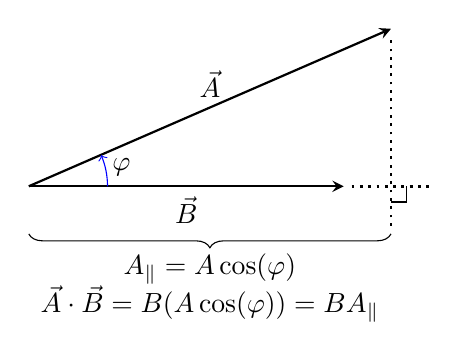
\begin{tikzpicture}[scale=2]
        \draw[->, thick, -stealth] (0,0)--node[below]{$\vec{B}$}(2,0);
        \draw[->, thick, -stealth] (0,0)--node[above]{$\vec{A}$}(2.3,1);
        \draw[line width=1pt,dotted] (2.05,0)--(2.55,0);
        \draw[line width=1pt,dotted] (2.3,-0.25)--(2.3,0.95);
        \draw[line width=0.5pt] (2.4,0)--(2.4,-0.1)--(2.3,-0.1);
        \draw [decorate,decoration={brace,amplitude=5pt,mirror,raise=4ex}](0,0)--(2.3,0) node[midway,yshift=-3em]{$A_{\parallel} = A\cos(\phi)$};
        \draw (0.6,0) coordinate (a);
        \draw (0.5, 0.215) coordinate (c);
        \draw (0,0) coordinate (b);
        \draw pic["$\phi$", draw=blue, ->, angle eccentricity=1.2, angle radius=1cm]{angle=a--b--c};
        \node at (1.15, -0.75){$\vec{A} \cdot \vec{B} = B(A\cos(\phi)) = BA_{\parallel}$};
    \end{tikzpicture}
    \end{center}
    Or as the product of $A$ with with the projection $B_{\parallel}$ of $\vec{B}$ onto the direction of $\vec{A}$
    \begin{center}
    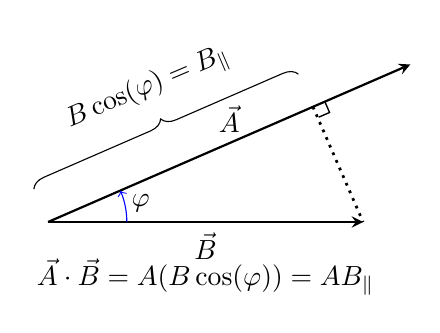
\begin{tikzpicture}[scale=2]
        \draw[->, thick, -stealth] (0,0)--node[below]{$\vec{B}$}(2,0);
        \draw[->, thick, -stealth] (0,0)--node[above]{$\vec{A}$}(2.3,1);
        \draw (0.6,0) coordinate (a);
        \draw (0.5, 0.215) coordinate (c);
        \draw (0,0) coordinate (b);
        \draw pic["$\phi$", draw=blue, ->, angle eccentricity=1.2, angle radius=1cm]{angle=a--b--c};            \draw (0,0) coordinate (aa);
        \draw (2.3,1) coordinate (bb);
        \draw (2,0) coordinate (cc);
        \draw (2.09,0) coordinate (dd);
        \draw[line width=1pt,dotted] ($(aa)!(cc)!(bb)$)--(cc);
        \draw [decorate,decoration={brace,amplitude=5pt,raise=3ex}](0,0)--($(aa)!(cc)!(bb)$) node[midway,rotate=23.1,yshift=3em]{$B\cos(\phi) = B_{\parallel}$};
        \node at (1,-0.35) {$\vec{A} \cdot \vec{B} = A(B\cos(\phi))=AB_{\parallel}$};
        \draw[line width=0.5pt] ($(aa)!(dd)!(bb)$)--([turn]-90:0.075cm)--([turn]-90:0.075cm);
    \end{tikzpicture}
    \end{center}

    The vector product of two vectors $\vec{A}$ and $\vec{B}$, ($\vec{A}\times\vec{B}$), is a vector that has its direction perpendicular to both vectors $\vec{A}$ and $\vec{B}$. vector $\vec{A}\times\vec{B}$ is perpendicular to the plane containing $\vec{A}$ and $\vec{B}$. The magnitude of the vector produced is $|\vec{A}\times\vec{B}|=AB\sin(\phi)$ where the angle $\phi$ is measured from the first vector ($\vec{A}$) to the second ($\vec{B}$) and is between $0\degree$ and $180\degree$. When $\phi = 0$, $\vec{A}\times\vec{B} = 0$, $(\sin(0\degree) = 0 = \sin(180\degree))$
    \begin{figure}
    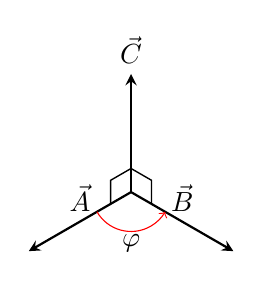
\begin{tikzpicture}[scale=1.5]
        \draw[->,thick,-stealth] (0,0)--(0,1)node[above]{$\vec{C}$};
        \draw[->,thick,-stealth] (0,0)--node[above]{$\vec{B}$}({cos(-30)},{sin(-30)});
        \draw[->,thick,-stealth] (0,0)--node[above]{$\vec{A}$}(-{cos(-30)},{sin(-30)});
        \draw[line width=0.5pt] (0,0.2)--({0.2*cos(-30)},-{0.2*sin(-30)})--({0.2*cos(-30)},{0.2*sin(-30)});
        \draw[line width=0.5pt] (0,0.2)--(-{0.2*cos(-30)},-{0.2*sin(-30)})--(-{0.2*cos(-30)},{0.2*sin(-30)});
        \draw (-{0.35*cos(-30)},{0.35*sin(-30)}) coordinate (a);
        \draw ({0.35*cos(-30)},{0.35*sin(-30)}) coordinate (b);
        \draw (0,0) coordinate (c);
        \draw pic["$\phi$", draw=red, ->, angle eccentricity=1.3, angle radius=0.5cm]{angle=a--c--b};
    \end{tikzpicture}
    \hskip 35pt
    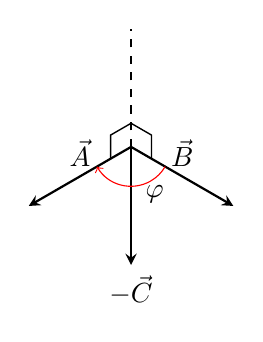
\begin{tikzpicture}[scale=1.5]
        \draw[line width=0.8pt,dashed] (0,0)--(0,1);
        \draw[->,thick,-stealth] (0,0)--(0,-1)node[below]{$-\vec{C}$};
        \draw[->,thick,-stealth] (0,0)--node[above]{$\vec{B}$}({cos(-30)},{sin(-30)});
        \draw[->,thick,-stealth] (0,0)--node[above]{$\vec{A}$}(-{cos(-30)},{sin(-30)});
        \draw[line width=0.5pt] (0,0.2)--({0.2*cos(-30)},-{0.2*sin(-30)})--({0.2*cos(-30)},{0.2*sin(-30)});
        \draw[line width=0.5pt] (0,0.2)--(-{0.2*cos(-30)},-{0.2*sin(-30)})--(-{0.2*cos(-30)},{0.2*sin(-30)});
        \draw (-{0.35*cos(-30)},{0.35*sin(-30)}) coordinate (a);
        \draw ({0.35*cos(-30)},{0.35*sin(-30)}) coordinate (b);
        \draw (0,0) coordinate (c);
        \draw pic[draw=red, <-, angle eccentricity=1.3, angle radius=0.5cm]{angle=a--c--b};
        \node at (0.2,-0.4){$\phi$};
    \end{tikzpicture}
    \end{figure}
\end{document}